% This is samplepaper.tex, a sample chapter demonstrating the
% LLNCS macro package for Springer Computer Science proceedings;
% Version 2.20 of 2017/10/04
%
\documentclass[runningheads]{llncs}
%
\usepackage{graphicx}
\usepackage{multirow}
\usepackage{amsmath}
\usepackage{wrapfig}
\usepackage{float}
% Used for displaying a sample figure. If possible, figure files should
% be included in EPS format.
%
% If you use the hyperref package, please uncomment the following line
% to display URLs in blue roman font according to Springer's eBook style:
% \renewcommand\UrlFont{\color{blue}\rmfamily}

\begin{document}
%
\title{Data mining techniques-Assignment 1}
%
%\titlerunning{Abbreviated paper title}
% If the paper title is too long for the running head, you can set
% an abbreviated paper title here
%
\author{Gongze Cao, Xinyu Fu}
%

\institute{VU-Group 66}

%
\maketitle              % typeset the header of the contribution
%
%
%
%
\section{Explore the dataset}

The dataset we consider there comes from the answer from 280 students to a designed questionnaire. This dataset has 16 entries of different types, one is date, another is time, the rest of them are either categorical or numerical/string. Categorical variables are simply represented by integers to facilitate the later analysis. There are 8 entries having missing values, determined by either the "unknown" answer or an invalid answer. The missing value and specs of each attribute is shown in the table below:

\begin{table}[]
    \begin{tabular}{llllll}
    Attribute  & Data Type & NumMissedVal & Attribute   & Data Type & NumMissedVal \\
    Program    & Str       & 0                    & Gender      & Int       & 4                    \\
    ML         & Cate       & 3                    & IR          & Cate       & 13                   \\
    Stats      & Cate       & 12                   & DB          & Int       & 6                    \\
    Neighbors  & Int       & 49                   & StressLevel & Int       & 1                    \\
    DM Compete & Int       & 61                   & Choco       & Cate       & 33                   \\
    Birthday   & Str       & 49                   & rand        & Int       & 16                   \\
    gd1        & Str       & 0                    & gd2         & Str       & 0                    \\
    bed time   & Str       & 0                    & stand up    & Cate       & 9                   
    \end{tabular}
\end{table}

\subsection{Preprocessing}
\label{sec:prep}

We select several attributes to further analysis, consisting of "Gender", "ML", "IR", "Stat", "DB", "Neighbors", "Stress level", "Program", "DM", as they are prune to contains information about the person and our further prediction task.

\subsubsection{Categorical}
Categorical data, such as "standup", "ML", "IR", are stored using integer as format, as most of them come from multiple choices, they are marked as missing value provided only specific option is chosen, such as "unknown". We ignore the missing value temporarily and assign them with the maximum option afterward when analysis.
\subsubsection{Numerical}
There are a few of numerical attributes either stored in Integer or Float way, for those attributes who has a specific range, such as "StressLevel" and "DM", we mark all entries falling out of this range to be the closest range margin before reading it. After read all entries regardless of the missing values, we assigned the missed value with the median. Specifically, for later analysis of the classification, we mark all entries with "StressLevel" greater than 50 to be label 1, and all entries with "StressLevel" smaller than 50 to be label 0, per intuition of human nature.
\subsubsection{String}
"Program" consists of many different strings inputted by the students, and we roughly classified all program to 10 classes, that is: "Artificial Intelligence", "Business", "Computational Science", "Computer Science", "Engineer", "Finance", "Information Science", "Others", "Physics", "QRM". After this we store this attribute in a one-hot way.

\subsubsection{General}
We drop the duplicate, normalize the data per attribute level after all the pervious processing is done. The final feature of all entries in all is (278, 17).

\subsection{Feature properties}
\subsubsection{Percentage}
The first thing we care about is the percentage of each property for an categorical variable, so as a warming up we plot a bar graph for the programs of all enrolled student:

\begin{figure}[h]
    \centering
    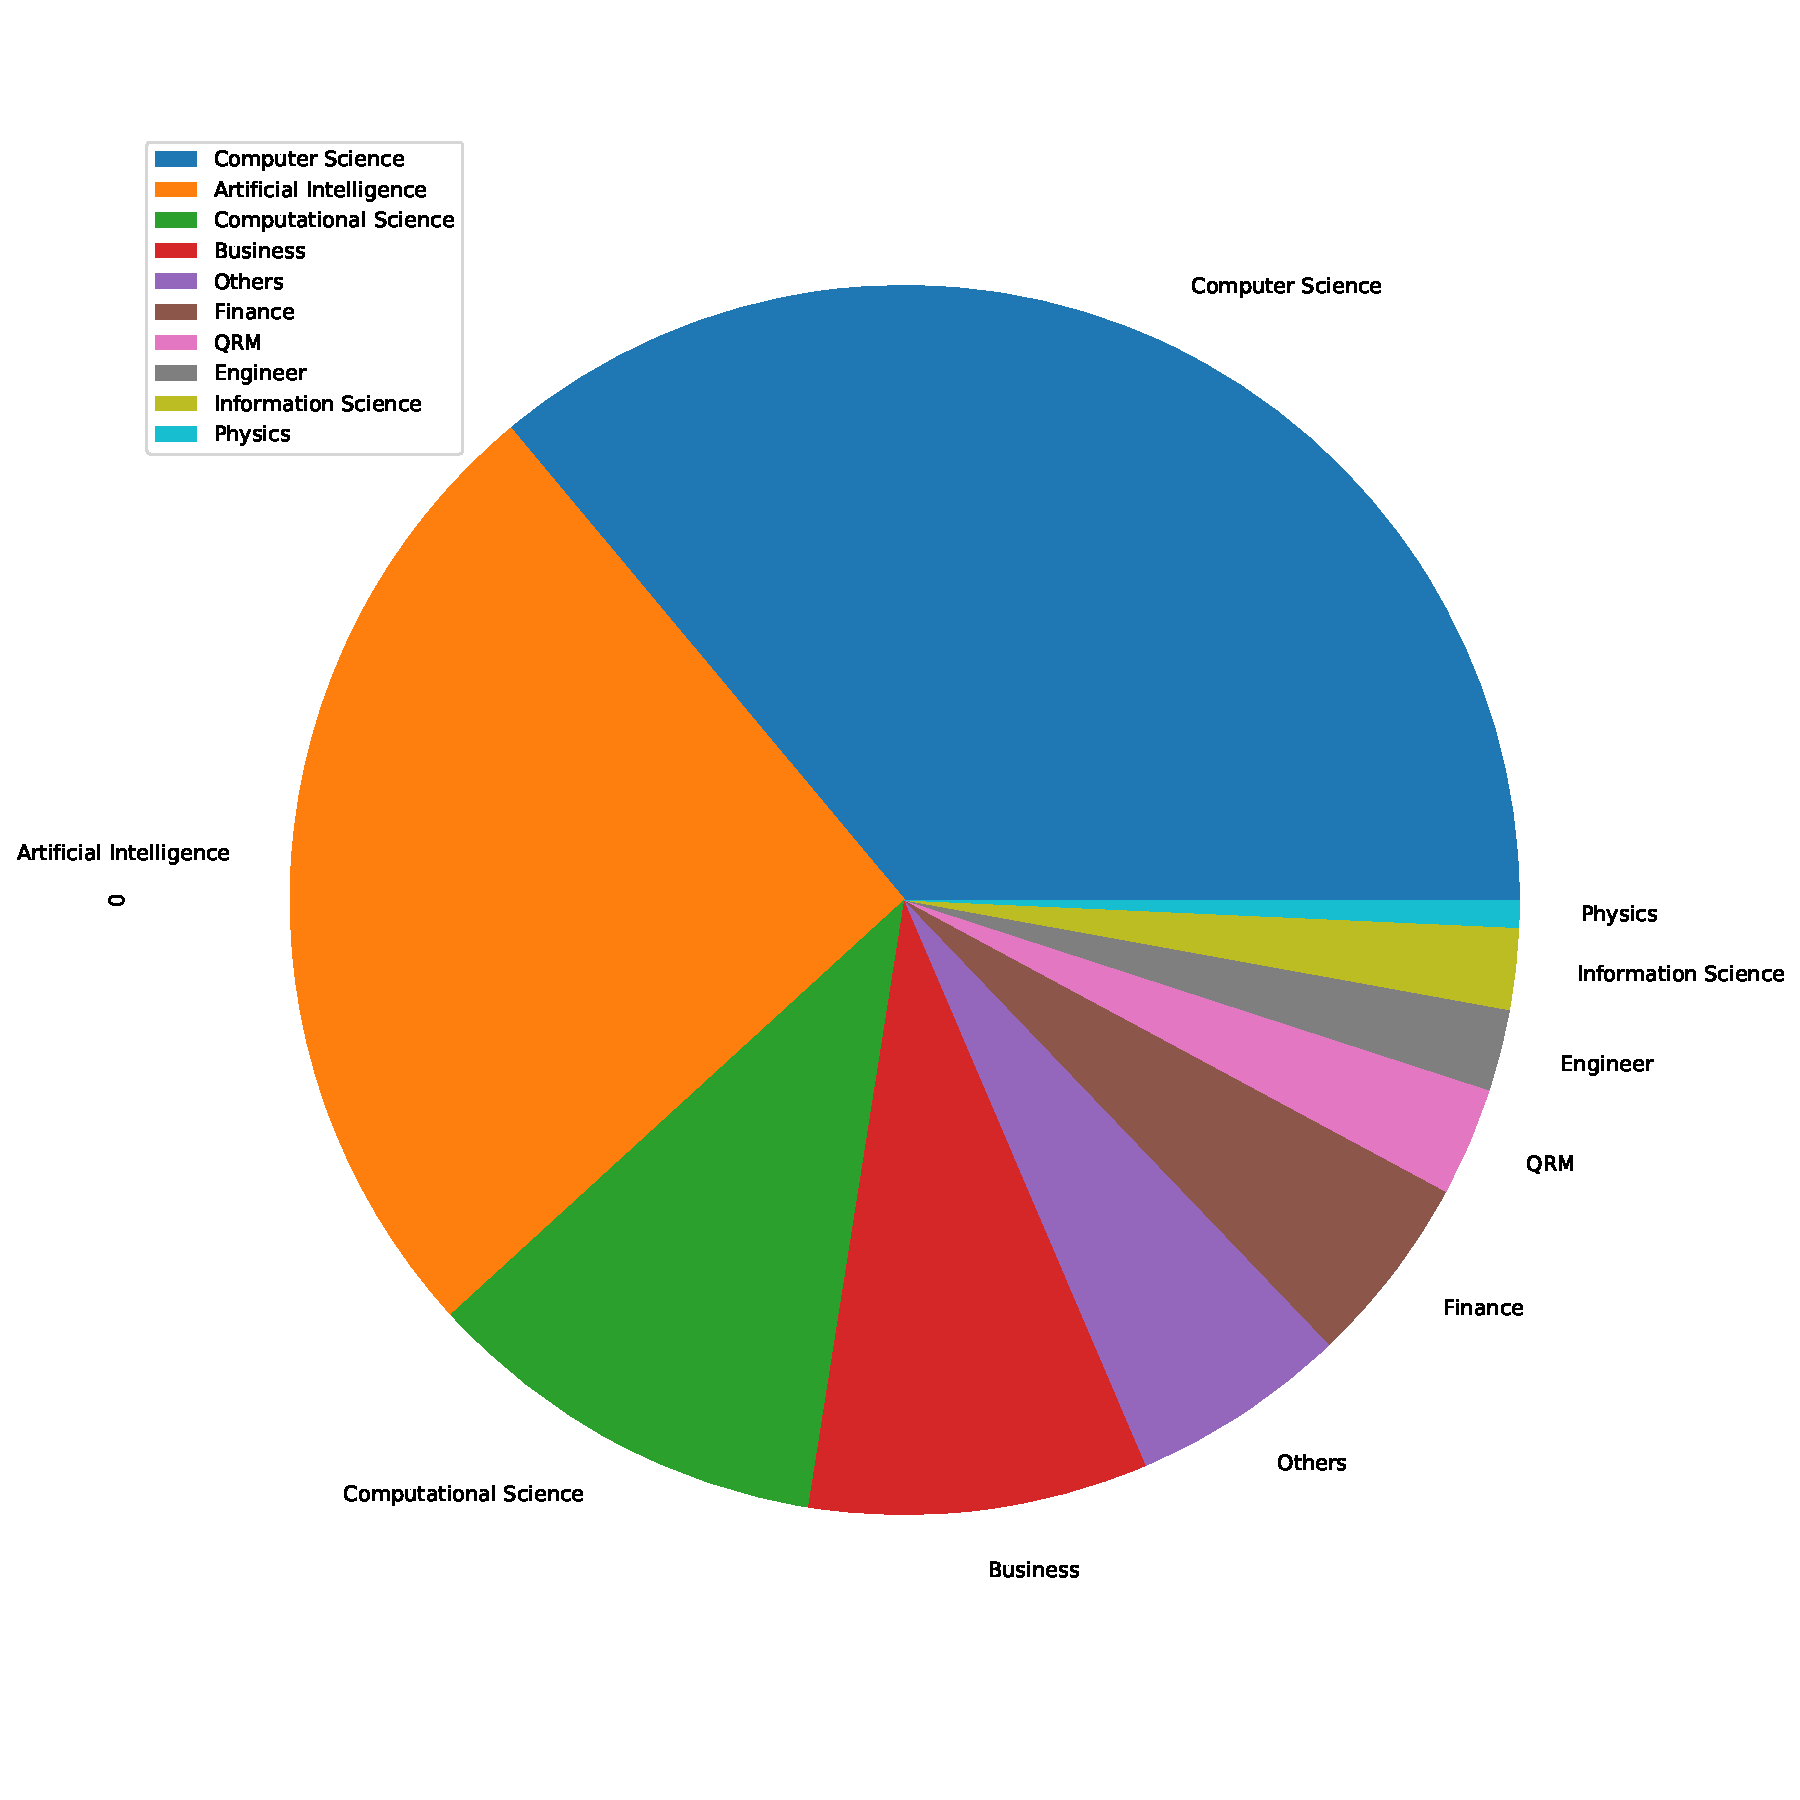
\includegraphics[width=6cm]{./images/pie_plot.pdf}
    \caption{The bar plot of the program distribution among all enrolled students. The top 3 most program is "Artificial Intelligence", "Computer Science" and "Computational science".}
    \label{fig:bar}
\end{figure}
\subsubsection{Description of statistics of all attributes}
We also show some of the most commonly used statistics of all attributes in this dataset:

\begin{table}[]
    \caption{The common data statistics upon all attributes.}
    \begin{tabular}{|c|c|c|c|c|c|c|c|}
    \hline
                  & gender & machine learning & information retrieval & Stat   & DB     & DM     & stress level \\ \hline
    mean          & 0.4307 & 0.6400           & 0.2981                & 0.8985 & 0.5294 & 0.2937 & 0.4207       \\ \hline
    std           & 0.4960 & 0.4808           & 0.4582                & 0.3025 & 0.5004 & 0.3632 & 0.2773       \\ \hline
    min           & 0.00   & 0.00             & 0.00                  & 0.00   & 0.00   & 0.00   & 0.00         \\ \hline
    max           & 1.00   & 1.00             & 1.00                  & 1.00   & 1.00   & 1.00   & 1.00         \\ \hline
    0.25 quantile & 0.00   & 0.00             & 0.00                  & 1.00   & 0.00   & 0.01   & 0.20         \\ \hline
    0.5 quantile  & 0.00   & 1.00             & 0.00                  & 1.00   & 1.00   & 0.10   & 0.40         \\ \hline
    0.75 quantile & 1.00   & 1.00             & 1.00                  & 1.00   & 1.00   & 0.50   & 0.65         \\ \hline
    \end{tabular}
    \end{table}
It is interesting to see that the median of stress level is around 0.40, meaning the major part of the students is not burnt, as it's not yet the final test. But meanwhile there is a quarter of students having "StressLevel" more than 0.65.

\subsubsection{Correlations}
We selected several attributes that shows relatively strong correlation and plotted their correlations and corresponding p-values into a plot as below:

\begin{figure}[h]
    \centering
    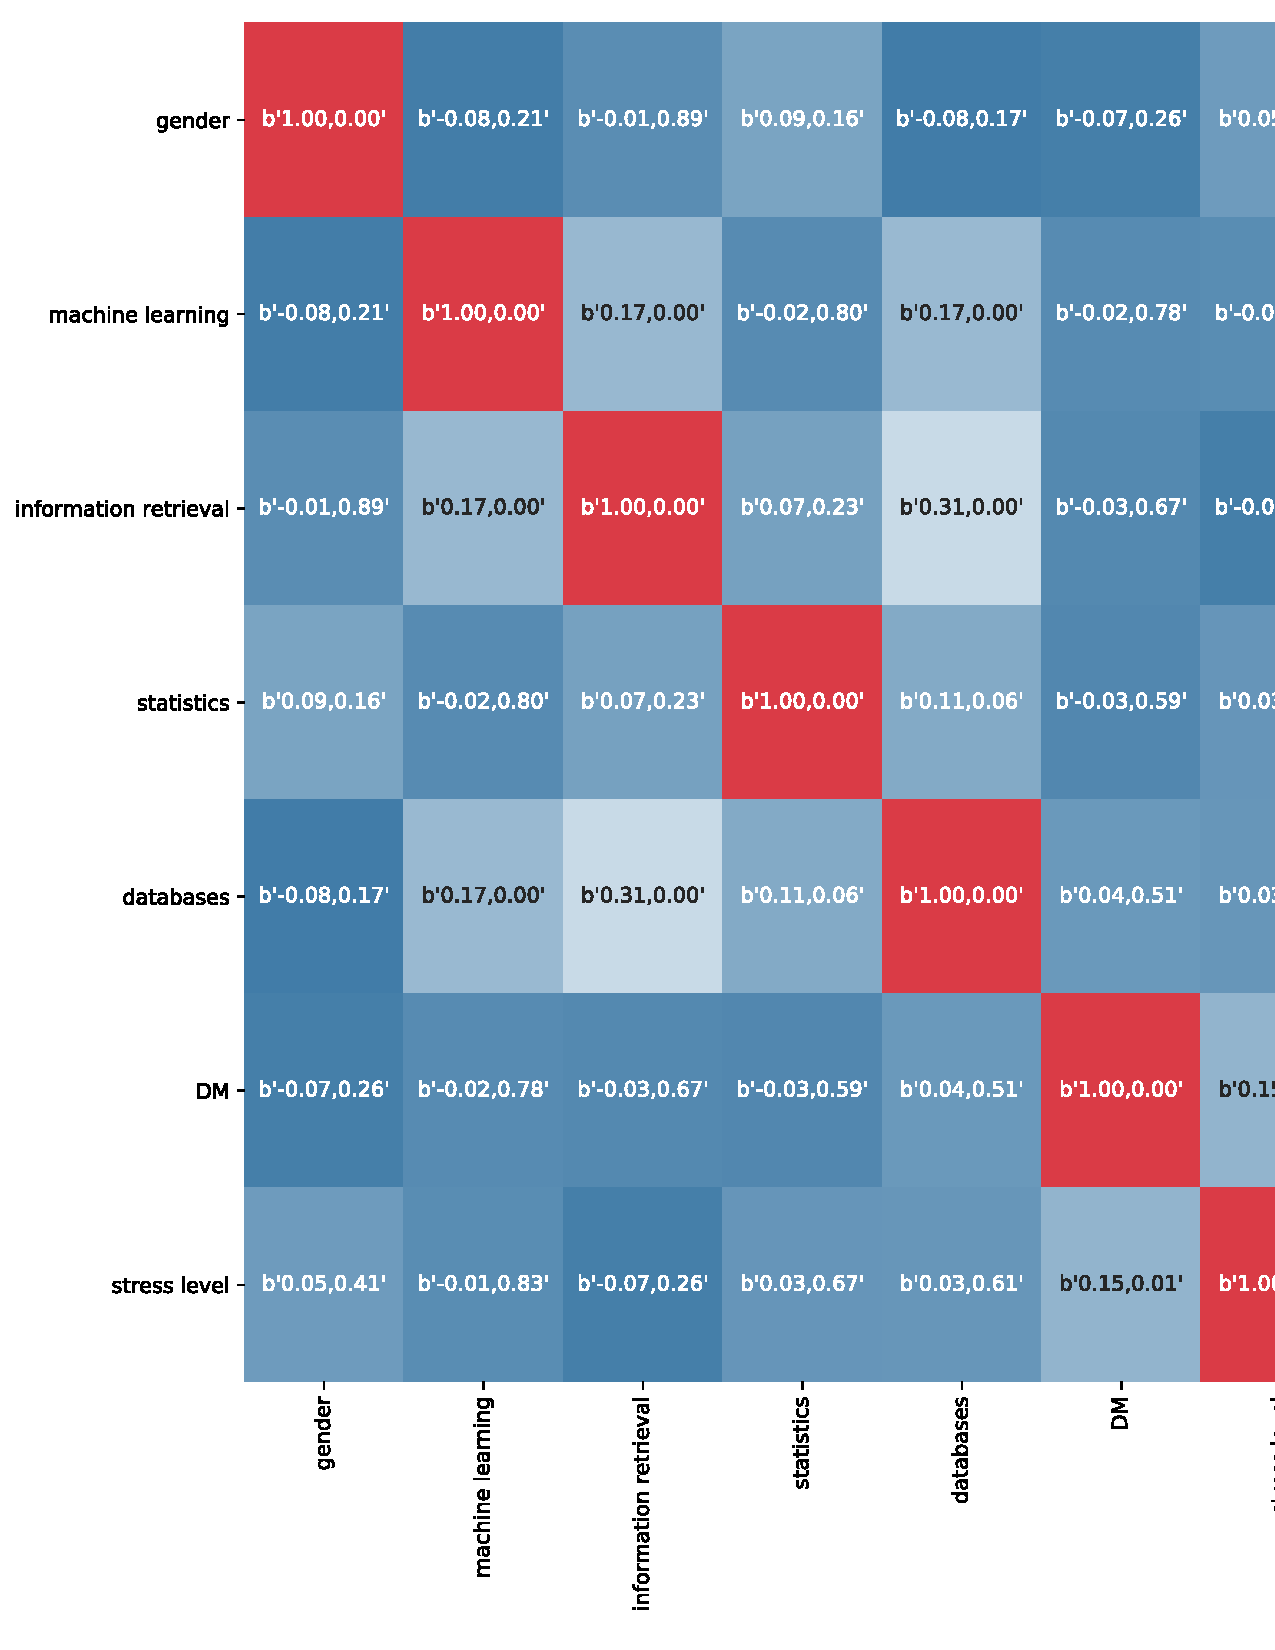
\includegraphics[width=6cm]{./images/corr_heatmap.pdf}
    \caption{Correlation coefficient and p-values for 7 features. If p-value is larger than 0.05 we can think the two variables are independent.}
    \label{fig:corr}
\end{figure}

We found that the "Machine Learning", "Information retrieval" and "Database" attributes have p-values smaller than 0.05 and are strongly correlated. While other attributes generally have p-values larger than 0.05 with every other attributes, so they are independent.

Specifically we are considering the sex ratio in every program involved, the following is a bar chart of showing the sex ratio of all program listed above:

\begin{figure}[h]
    \centering
    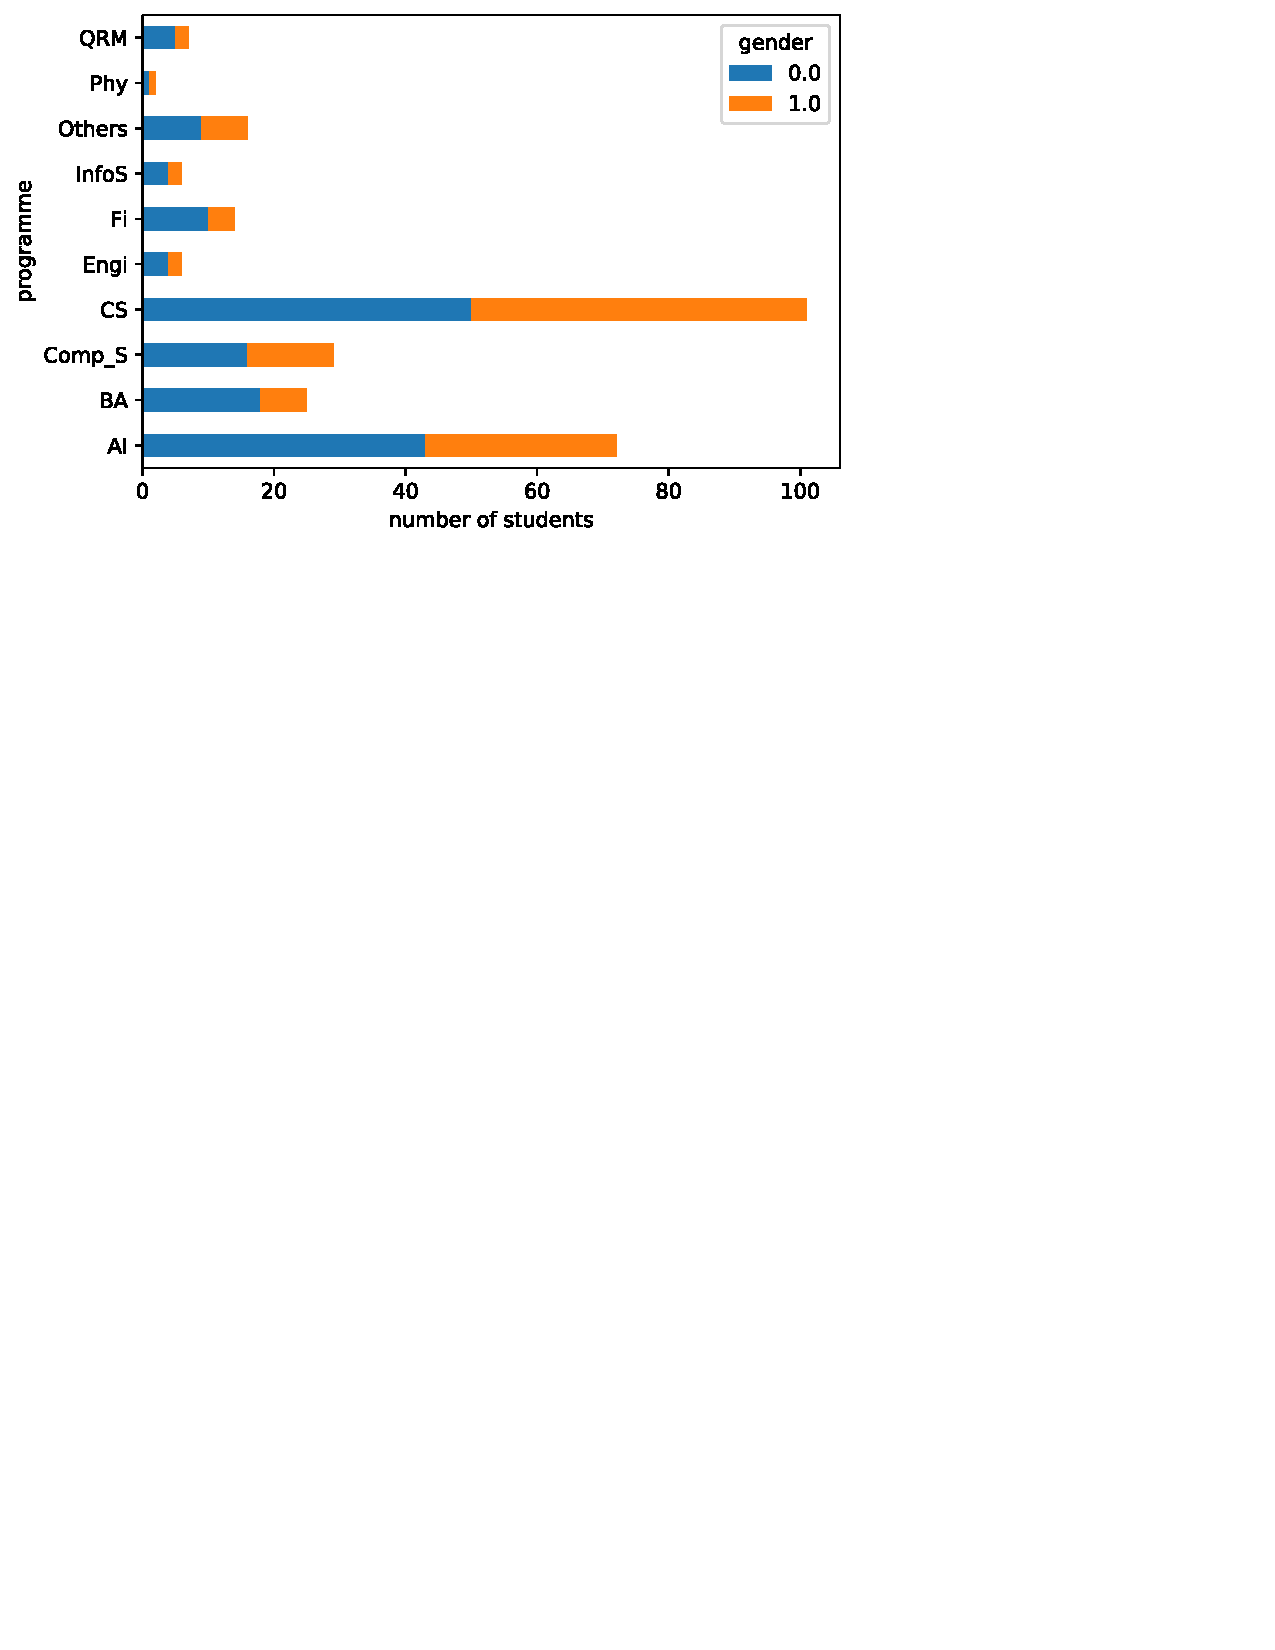
\includegraphics[width=10cm]{./images/genders.pdf}
    \caption{The bar chart of all genders ratio in every program, where 0.0 stands for male students and 1.0 stands for the female students.}
    \label{fig:gender}
\end{figure}

We found that in almost all program the male students are more than the female students. But for the largest program involved, Computer Science, the male students and female ones are of almost equal number.


% \subsubsection{Description of statistics of all attributes}
\subsection{Classification}
\label{sec:clf}
The task we are interested is whether we could infer the stresslevel of the student using other features. The feature set we choose is:"program" "gender","machine learning", "information retrieval","statistics","databases","DM". The label comes from the way stated in \ref{sec:prep}. We try with several different classifier and tune the hyper-parameters based on the cross-validation accuracy, and we choose the fold to be 5 and fixed for all classifiers.\\ The results are shown below:
\begin{table}[]
    \centering
    \caption{The maximum validation accuracy of all classifiers through experiments.}
    \begin{tabular}{|l|l|l|l|l|l|l|l|}
        \hline
        Classifier & LR    & KNN   & GBDT  & RF    & SVM   & GNB   & DT    \\ \hline
        Accuracy & 0.546 & 0.546 & 0.615 & 0.600 & 0.579 & 0.557 & 0.593 \\ \hline
    \end{tabular}
    \label{fig:gender}
\end{table}
For Linear Regression(LR), among penalty=["l1", "l2"], C=[0.1, 1, 10], we choose penalty="l1" and C="10". Since the feature might be redundant, so we tend to choose a larger C at the begimning and the results seem to align with the observation. We also hypothesize that l1 penalty might lead to more generalized model, but the experiments shows l1 and l2 penalty differs little.

From the experience of LR, we use C=100 when training SVM and it gives boosted performance in terms of Cross-validation accuracy.

For KNN classifier, among k=[1,2,3,4,5,6] we empirically choose k=6 as it gives better cross-validation accuracy. We think the larger k might suffer from over-smoothing.

For decision tree, among max-depth=[1,2,3,4,5,6], we empirically find smaller depth lead to better generalization performance, when depth=2 the train-valid tradeoff is optimized.

For Gradiant-boosting-decision-tree(GBDT) and Random Forest(RF), from the experience of decision tree above, we choose smaller max-depth again and it leads to good performance. For GBDT we used 20 base estimators and 2 as max-depth, for RF we used 200 base estimators and 4 as max-depth.

For Gaussian Naive classifier we used the default setup as a baseline.

In general, the GBDT works the best and used much less parameters than its opponent RF. It might indicate the sturcture of GBDT fits better for this kind problem than any other classifier.



\section{Research and theory}

\subsection{Theory: Analyze a less obvious dataset}
\begin{itemize}
    
    \item Firstly do some cleaning on the given dataset. We extract the labels of the dataset by convert the first word from "ham" to 1 and "spam" to 0. Then we use the text after the label as the raw feature. After filtering out all punctuation in the raw feature, we used TF-IDF to transform the raw feature to a numerical vector of size (9534,). The final shape of the feature matrix and label are (5574, 9534) and (5574,) respectably.
    \item We then trained 6 classifiers as did in section \ref{sec:clf}, the cross validation fold is set again as 5 and results are shown in the table below:
    \begin{table}[]
        \centering
        \caption{The cross validation accuracy of all classifiers through experiments on SmsCollection.}
        \begin{tabular}{|l|l|l|l|l|l|l|l|}
            \hline
            Classifier & LR    & KNN   & GBDT  & RF    & SVM     & DT    \\ \hline
            Accuracy & 0.956 & 0.927 & 0.966 & 0.970 & 0.866  & 0.959 \\ \hline
        \end{tabular}
        \label{fig:clf2}
    \end{table}
\end{itemize}
All the classifiers use the default parameters provided by the sklearn. We did not perform further tuning as the performance is already very impressive. Among all the classifiers the decision tree based classifiers perform the best, GBDT, RF and DT all achieve validation accuracy above 95 percents. To further improve the performance we advice not only further tuning with the base estimators number and max depth in DT-based classifiers, but also include more linear classifiers and create a boosting mega classifier.

% %
% % ---- Bibliography ----
% %
% % BibTeX users should specify bibliography style 'splncs04'.
% % References will then be sorted and formatted in the correct style.
% %
% % \bibliographystyle{splncs04}
% % \bibliography{mybibliography}
% %
% \begin{thebibliography}{8}
% \bibitem{ref_article1}
% Xudong Liu, Bing Xu, Yuyu Zhang, "Combination of Diverse Ranking Models for Personalized Expedia Hotel Searches".

% \bibitem{ref_article2}
% Xin Xing, Yao Xiao, Shunji Li, "Personalized Expedia Hotel Searches", Stanford University.

% \bibitem{ref_article3}
% Saurabh Agarwal, Luke Styles, Saurabh Verma, "Learn to Rank ICDM 2013 Challeng Ranking Hotel Search Queries".

% \end{thebibliography}
\end{document}
